\documentclass[sigconf]{acmart}

\usepackage{booktabs} % For formal tables
\usepackage{epstopdf} % For eps
\usepackage{url}
\usepackage[T1]{fontenc}
\usepackage{float}

% Copyright
%\setcopyright{none}
%\setcopyright{acmcopyright}
%\setcopyright{acmlicensed}
\setcopyright{rightsretained}
%\setcopyright{usgov}
%\setcopyright{usgovmixed}
%\setcopyright{cagov}
%\setcopyright{cagovmixed}


% DOI
\acmDOI{XX.XXX/XXX_X}

% ISBN
\acmISBN{XXX-XXXX-XX-XXX/XX/XX}

%Conference
\acmConference[WebMedia'2017]{Brazilian Symposium on Multimedia and the Web}{October 2017}{Gramado, RS Brazil} 
\acmYear{2017}
\copyrightyear{2017}

\acmPrice{15.00}


\begin{document}
\title{CrowdNote}
%\titlenote{Produces the permission block, and
 % copyright information}
\subtitle{Crowdsourcing Environment for Complex Video Annotations}
%\subtitlenote{The full version of the author's guide is available as
%  \texttt{acmart.pdf} document}


\author{Removed for double-blind review}
%\authornote{Dr.~Trovato insisted his name be first.}
%\orcid{1234-5678-9012}
\affiliation{%
  \institution{Removed for double-blind review}
%  \streetaddress{Removed for double-blind review}
 % \city{Removed for double-blind review} 
  %\state{Removed for double-blind review} 
  %\postcode{Removed for double-blind review}
}
\email{Removed-for-double-blind-review}

\author{Removed for double-blind review}
%\authornote{Dr.~Trovato insisted his name be first.}
%\orcid{1234-5678-9012}
\affiliation{%
  \institution{Removed for double-blind review}
 % \streetaddress{Removed for double-blind review}
  %\city{Removed for double-blind review} 
  %\state{Removed for double-blind review} 
  %\postcode{Removed for double-blind review}
}
\email{Removed-for-double-blind-review}

\author{Removed for double-blind review}
%\authornote{Dr.~Trovato insisted his name be first.}
%\orcid{1234-5678-9012}
\affiliation{%
  \institution{Removed for double-blind review}
  %\streetaddress{Removed for double-blind review}
  %\city{Removed for double-blind review} 
 % \state{Removed for double-blind review} 
 % \postcode{Removed for double-blind review}
}
\email{Removed-for-double-blind-review}



% The default list of authors is too long for headers}
\renewcommand{\shortauthors}{Removed for double-blind review}


\begin{abstract}
	This paper introduces CrowdNote, a crowdsourcing environment for complex video annotations without the need for trained workers or specialists. CrowdNote is based on a cascading microtasks approach to achieve complex video annotation by aggregating and processing multiple simple annotations collected from the crowd. The used approach consists of dividing complex annotation tasks into simple and small microtasks, and cascading them to generate a final result. Moreover, this approach allows to use simple annotation tools rather than complex and expensive annotation systems, also it tends to avoid activities that may be tedious and time-consuming for contributors, that are the workers in crowdsourcing scenarios. The CrowdNote instance presented in this paper produces enriched videos in which all extra content added is provided, selected and positioned by the crowd. However, this software is open source and can be downloaded and used as template for different crowdsourcing applications based on video annotation.

\end{abstract}

%
% The code below should be generated by the tool at
% http://dl.acm.org/ccs.cfm
% Please copy and paste the code instead of the example below. 
%
\begin{CCSXML}
<ccs2012>
<concept>
<concept_id>10002951.10003260.10003282.10003296</concept_id>
<concept_desc>Information systems~Crowdsourcing</concept_desc>
<concept_significance>500</concept_significance>
</concept>
<concept>
<concept_id>10003120.10003130.10003131.10003570</concept_id>
<concept_desc>Human-centered computing~Computer supported cooperative work</concept_desc>
<concept_significance>500</concept_significance>
</concept>
<concept>
<concept_id>10010405.10010497.10010510.10010513</concept_id>
<concept_desc>Applied computing~Annotation</concept_desc>
<concept_significance>500</concept_significance>
</concept>
<concept>
<concept_id>10002951.10003227.10003251</concept_id>
<concept_desc>Information systems~Multimedia information systems</concept_desc>
<concept_significance>500</concept_significance>
</concept>
<concept>
<concept_id>10003120.10003121.10003124.10010868</concept_id>
<concept_desc>Human-centered computing~Web-based interaction</concept_desc>
<concept_significance>500</concept_significance>
</concept>
</ccs2012>
\end{CCSXML}

\ccsdesc[500]{Information systems~Multimedia information systems}
\ccsdesc[500]{Human-centered computing~Web-based interaction}
\ccsdesc[500]{Information systems~Crowdsourcing}
\ccsdesc[500]{Human-centered computing~Computer supported cooperative work}
\ccsdesc[500]{Applied computing~Annotation}

\keywords{Crowdsourcing, Video Annotation, Human Computation, Microtasks, Multimedia Systems, Video Enrichment}

\maketitle

\section{Introduction}
	Video is a very effective information container and it is a highly expressive type of media, capable of providing a large semantic load by presenting different audiovisual components coherently\cite{162960}. However, video can be considerably more useful when carrying metadata that can be used by video applications, and are often represented as video annotations.

Video annotation involves inserting tags into video objects to describe their content and context, also to describing media characteristics such as quality, coding, among other features \cite{Wang:2009:BDM:1652990.1653002}. In other words, they are used to facilitate the work of users and systems that can handle annotated items.

Annotations facilitate the manipulation of videos, allowing the creation of content-based distribution applications \cite{Zhang:2012:KIE:2339530.2339620}, indexing \cite{Zhang:2007:PRS:1290082.1290126}, summarization \cite{Fiao:2016:AGS:3001773.3001802}, navigation \cite{Goldman:2008}, composition \cite{Wilk:2015:VCC:2713168.2713178}, among many others by both automatic and manual means \cite{Wang:2011:ALM:1899412.1899414}. In other words, they are used to facilitate the work of users and systems that can handle annotated items.

In this paper, video annotations are categorized as simple and complex ones, considering that simple annotations are those that can be acquired with a simple interaction of the workers in a microtask. In addition, a complex annotation is one that requires the worker execute a more tedious, hard or time-consuming task, in which he needs to perform multiple interactions. 

A frequent problem of using a crowdsourcing approach to video annotation is to balance the relation between task complexity and cost. Simple annotation tasks, such as clicking an object on a video, can be done in a few seconds for anyone, otherwise, more complex tasks such as providing complementary content and positioning it in the right position on a video, require some expertise of contributors and are more costly to them. In a crowdsourcing context, microtask is an ubiquitous designation for simple tasks that can be performed for any contributor quick and easily \cite{Difallah:2015:DMC:2736277.2741685}.

CrowdNote is a crowdsourcing environment capable to achieve complex video annotation without the need for specialized nor trained workers, and it can be used as template to build different crowdsourcing applications based on video annotation. The system presented in this paper is a CrowdNote instance that produces enriched versions of videos in which are incorporated extra content such as images, text boxes, Wikipedia content and Youtube videos. 

The remaining of this paper is structured as follows. Section 2 presents the CrowdNote architecture. Section 3 presents the CrowdNote instance for video enrichmen. Finally, section 4 concludes the paper presenting final considerations.


\section{Architecture}	
	CrowdNote was developed as a classic Web system. To facilitate the sharing of software produced, only technologies that do not require complex infrastructure were adopted. The server was fully developed in NodeJS for easy deployment, the client was developed in HTML 5 to improve compatibility and the persistence layer uses MongoDB as No-SQL database.

The architecture of the CrowdNote is illustrated in Figure~\ref{architecture} in which is possible observe the 3 main components: Server, Database and Clients.

\begin{figure}[h!]
	\centerline{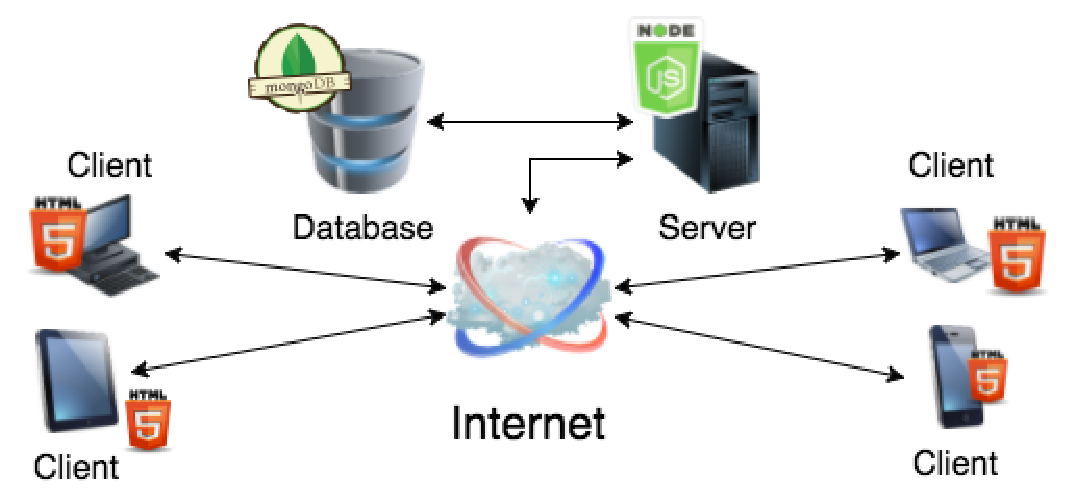
\includegraphics[scale=0.3] {figure/Architecture}}
	\caption{CrowdNote Architecture}
	\label{architecture}
\end{figure}

\subsection{Persistence}
The persistence was addressed using MongoDB, that deliver a very interesting solution to build No-SQL databases with some characteristics that meets the crowdsourcing requirements such as: high write load, high availability in an unreliable environment,  easy scaling and partition, heterogeneous data into the same collection.

In this model, JSON document collections are used instead of tables, and the documents in each collection may have a different structure to store different attributes. This feature allowed the modeling of a very simple database structure, composed of 3 collections of documents, as can be seen in Figure~\ref{persistence}. It was possible because documents in the Input and Output collections can contain different fields according to the task that consumes or generates the entries.

The Video collection stores entries related to the video segments dataset, the Input collection stores the input entries to the tasks, and the Output collection stores the contributions collected from the crowd.

\begin{figure}[h]
	\centerline{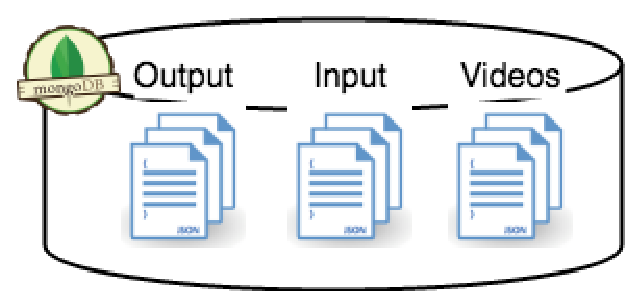
\includegraphics[scale=0.3] {figure/Persistence}}
	\caption{No-SQL Database - JSON Documents Collections}
	\label{persistence}
\end{figure}


\subsection{Workflow}

The internal workflow followed by CrowdNote is ilustrated by Figure~\ref{workflow}. The server system is composed by 3 modules: Collector, Aggregator and Player Provider.

\begin{figure}[h]
	\centerline{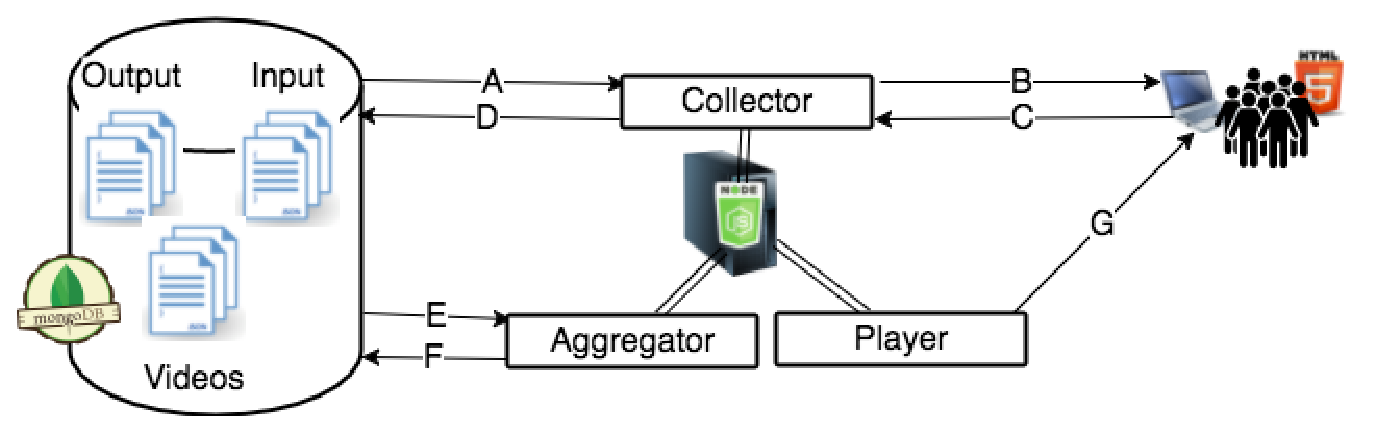
\includegraphics[scale=0.4] {figure/Workflow}}
	\caption{CrowdNote Workflow}
	\label{workflow}
\end{figure}

\textbf{Collector: } For each job request from the client, the Collector receive a register from the Input collection, that defines the annotation to be collected, and the respective media from the video collection (\textbf{A}). These information is used to generate the job view that sends it to a client (\textbf{B}) that renders it. A worker execute the job and this contribution is sent to Collector (\textbf{C}). Finally, the Collector store the contribution into the Output collection (\textbf{D}).

\textbf{Aggregator: } When a task is finished, the Aggregator receive all contributions into the Output collection related with that task (\textbf{E}). Aggregator applies the rules defines for the task to verify and process the contributions, so the result entries are stored into the Input collection (\textbf{F}), and these entries will be the new input to the next task.

\textbf{Player Provider: } When the Aggregator process the contributions for the last task, the result entries are stored into the Input collection as input for the Player Provider. This component sends to client instances the media and meta-data required to play the enriched videos (\textbf{G}).



\section{Video Enrichment Instance}
	To demonstrate how CrowdNote works, an instance was created to enrich the videos by incorporating extra content such as images, text boxes, Wikipedia content, and Youtube videos. In order to enrich the videos, it was decided that the crowd should to identify which points of interest in the video, suggest content to associate with them, select the best suggestions, and finally determine the position in the videos where they should be displayed.

Thus, 4 simple microtasks of annotation were defined, which when cascaded would generate the complex annotations necessary for enrichment. These annotations consist of the list of content that should be displayed in each interval of the video, as well as the position in which they should be displayed. In addition, for each microtask, was defined the appropriate aggregation method to generate input for the next one, as so to generate the final outcome.


\begin{itemize}
\item \textbf{Task 1 - Identify the points of interest} on the video that should be associated with extra content. The aggregation method proceed a temporal grouping over the contributions. For each group, a content analysis is performed to merge equivalent contributions. Finally, the predominant entry is selected in each group, and marked as the point of interest at that time in relation to the timeline.

\item \textbf{Task 2: Provide extra content suggestions} for each point of interest. In the aggregation, the content provided by contributors is grouped by point of interest. Therefore, a content analysis is done to group equivalent contributions.

\item \textbf{Task 3: Ranking the suggested content} provided by each point of interest. The contributors elect the suggested content that better complement each point of interest. In the aggregation, the most popular suggestion for each point of interest is selected based on contributions to task 3.
	
\item \textbf{Task 4: Determine the positions} to display the extra content associated with each point of interest. The contributors suggest the position for each content and, in the aggregation, the contributions are grouped by point of interest and, for each point, the average coordinate is determined.

\end{itemize}

\subsection{Cascading Microtasks}
The adopted approach consists in divide the complex annotation into simple annotations that can be collected by 
a set of simple annotation tools. Each of these simple annotations are collected by a microtask.

How is illustrated in Figure~\ref{cascading}, the input for each task is generated by the Aggregator after the previous task, except for the task 1. For this task is provided a bootstrap Input that is a list of video segments provided by the owner, that is who initiate the process. Each entry of the bootstrap input can represent a semantic block of the video. 

\begin{figure}[h!]
 \centerline{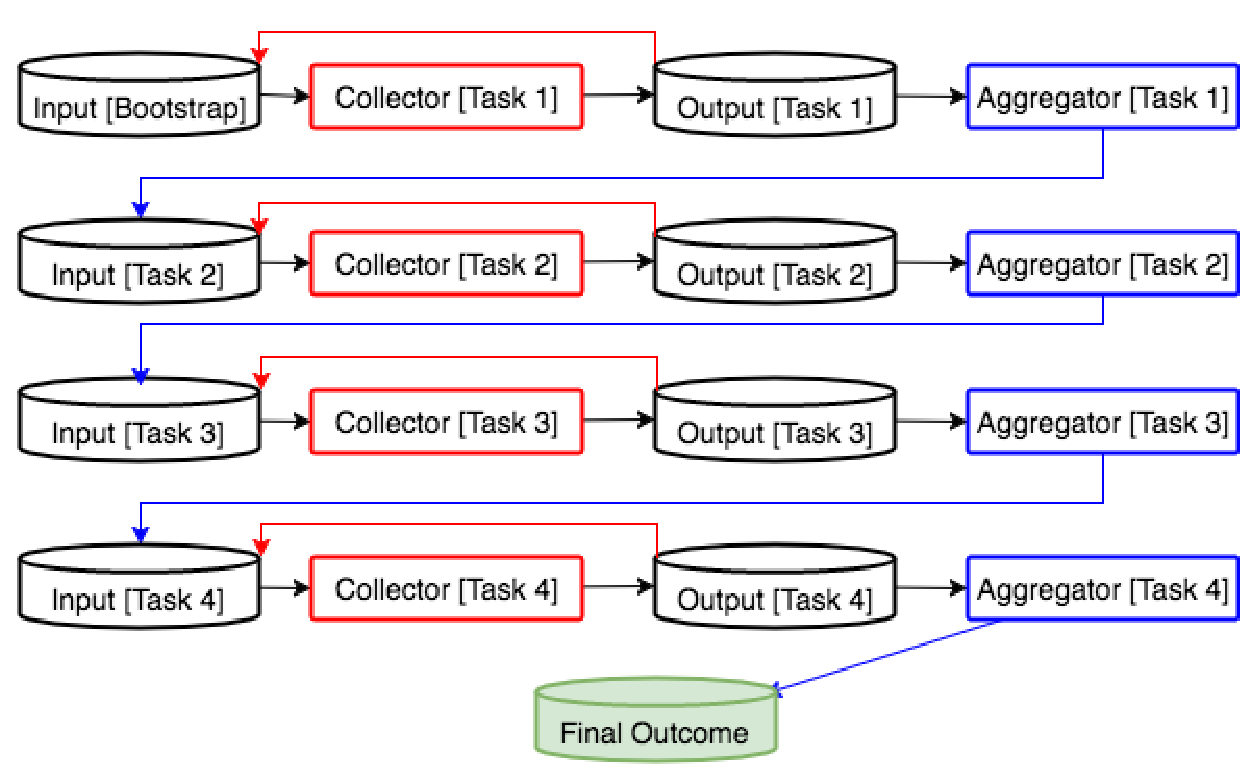
\includegraphics[scale=0.35] {figure/Cascading}}
	\caption{Cascading Microtasks}
	\label{cascading}
\end{figure}

Other applications that use CrowdNote may use different strategies to segment videos such as fixed time-length, SRT files, or even add a microtask to segment videos.
		


\subsection{Task 1}
\textbf{Identify Points of Interest:} The first annotation microtask is supported by the tool represented in Figure~\ref{task_1}, collecting identification for points of interest. In this task the contributor receive a segment of video that should be watched, and if was found any point of interest, it should be marked and briefly described. These points of interest can be gestures, words, expressions, facts, concept, characters, events or anything that can be related to extra content.

\begin{figure}[h!]
	\centerline{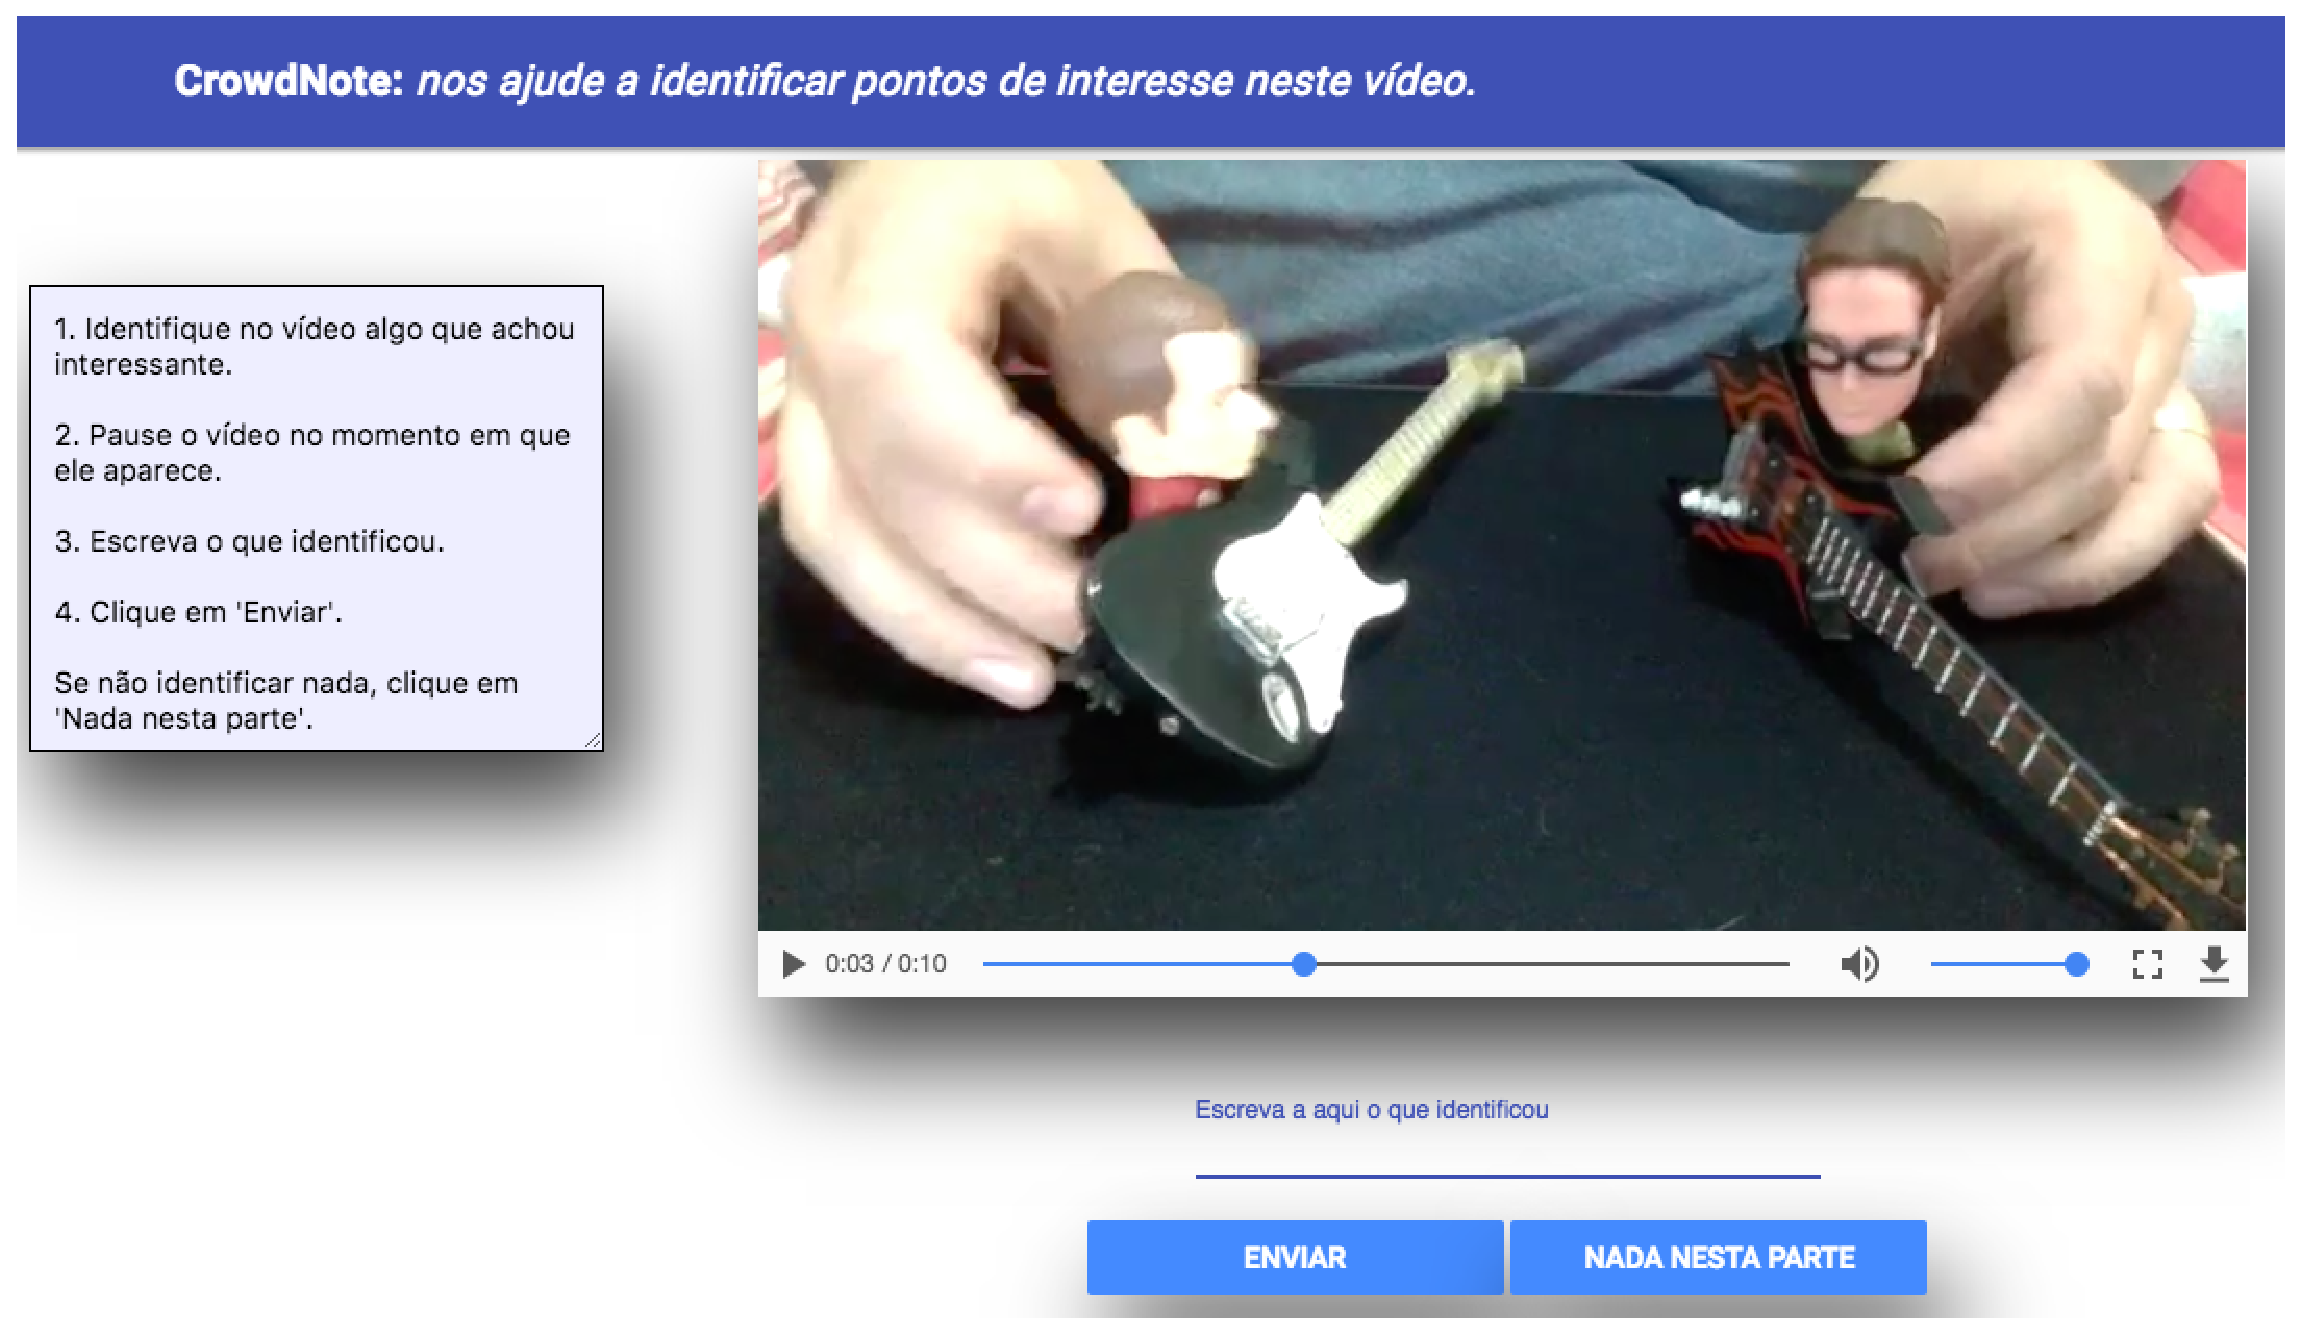
\includegraphics[scale=0.22] {figure/task_1}}
	\caption{Task 1}
	\label{task_1}
\end{figure}

\subsection{Task 2}

\textbf{Provide extra content suggestions:} The second task taken as input the aggregated result from the task 1 and is supported by the annotation tool represented in Figure~\ref{task_2}. In this task the contributor receive a video segment and a text describing  the point of interest to be observed, and must suggest an extra content to be associated with the point of interest. The extra content can be an image, a text, a hyperlink for a Youtube video, or a hyperlink to a Wikipedia page. 

\begin{figure}[h!]
	\centerline{\includegraphics[scale=0.18] {figure/task_2}}
	\caption{Task 2}
	\label{task_2}
\end{figure}

After the aggregation the outcome from this task is a set of points of interest, and a list of suggests of extra content to be related to each one of them.


\subsection{Task 3}

\textbf{Ranking Suggestions:} The third microtask aimed ranking the suggested contents that resulted from the task 2. The job consists in presenting to the worker a point of interest and the suggested contents related to it. The worker must select which content seems most appropriate to determine the point of interest. This task is supported by the annotation tool represented in Figure~\ref{task_3}.

		
\begin{figure}[h!]
	\centerline{\includegraphics[scale=0.22] {figure/task_3}}
	\caption{Task 3}
	\label{task_3}
\end{figure}

The aggregation process for this task checks which suggestions are most popular among the contributors and selects them to enrich the video.

\subsection{Task 4}

\textbf{Determine the positions:} The last task is to determine the position in the video where the extra content for each point of interest should be displayed. The correct position of each extra content is important to avoid occlusion and display content pleasingly to the user.

Following the studies about wisdom  of the crowd, the strategy to determine the correct position is to calculate the average coordinate of the contribution for each content \citep{GALTON1907}. The annotation tool represented in Figure~\ref{task_4} made this microtask faster and easier between the 4 tasks.

\begin{figure}[h!]
	\centerline{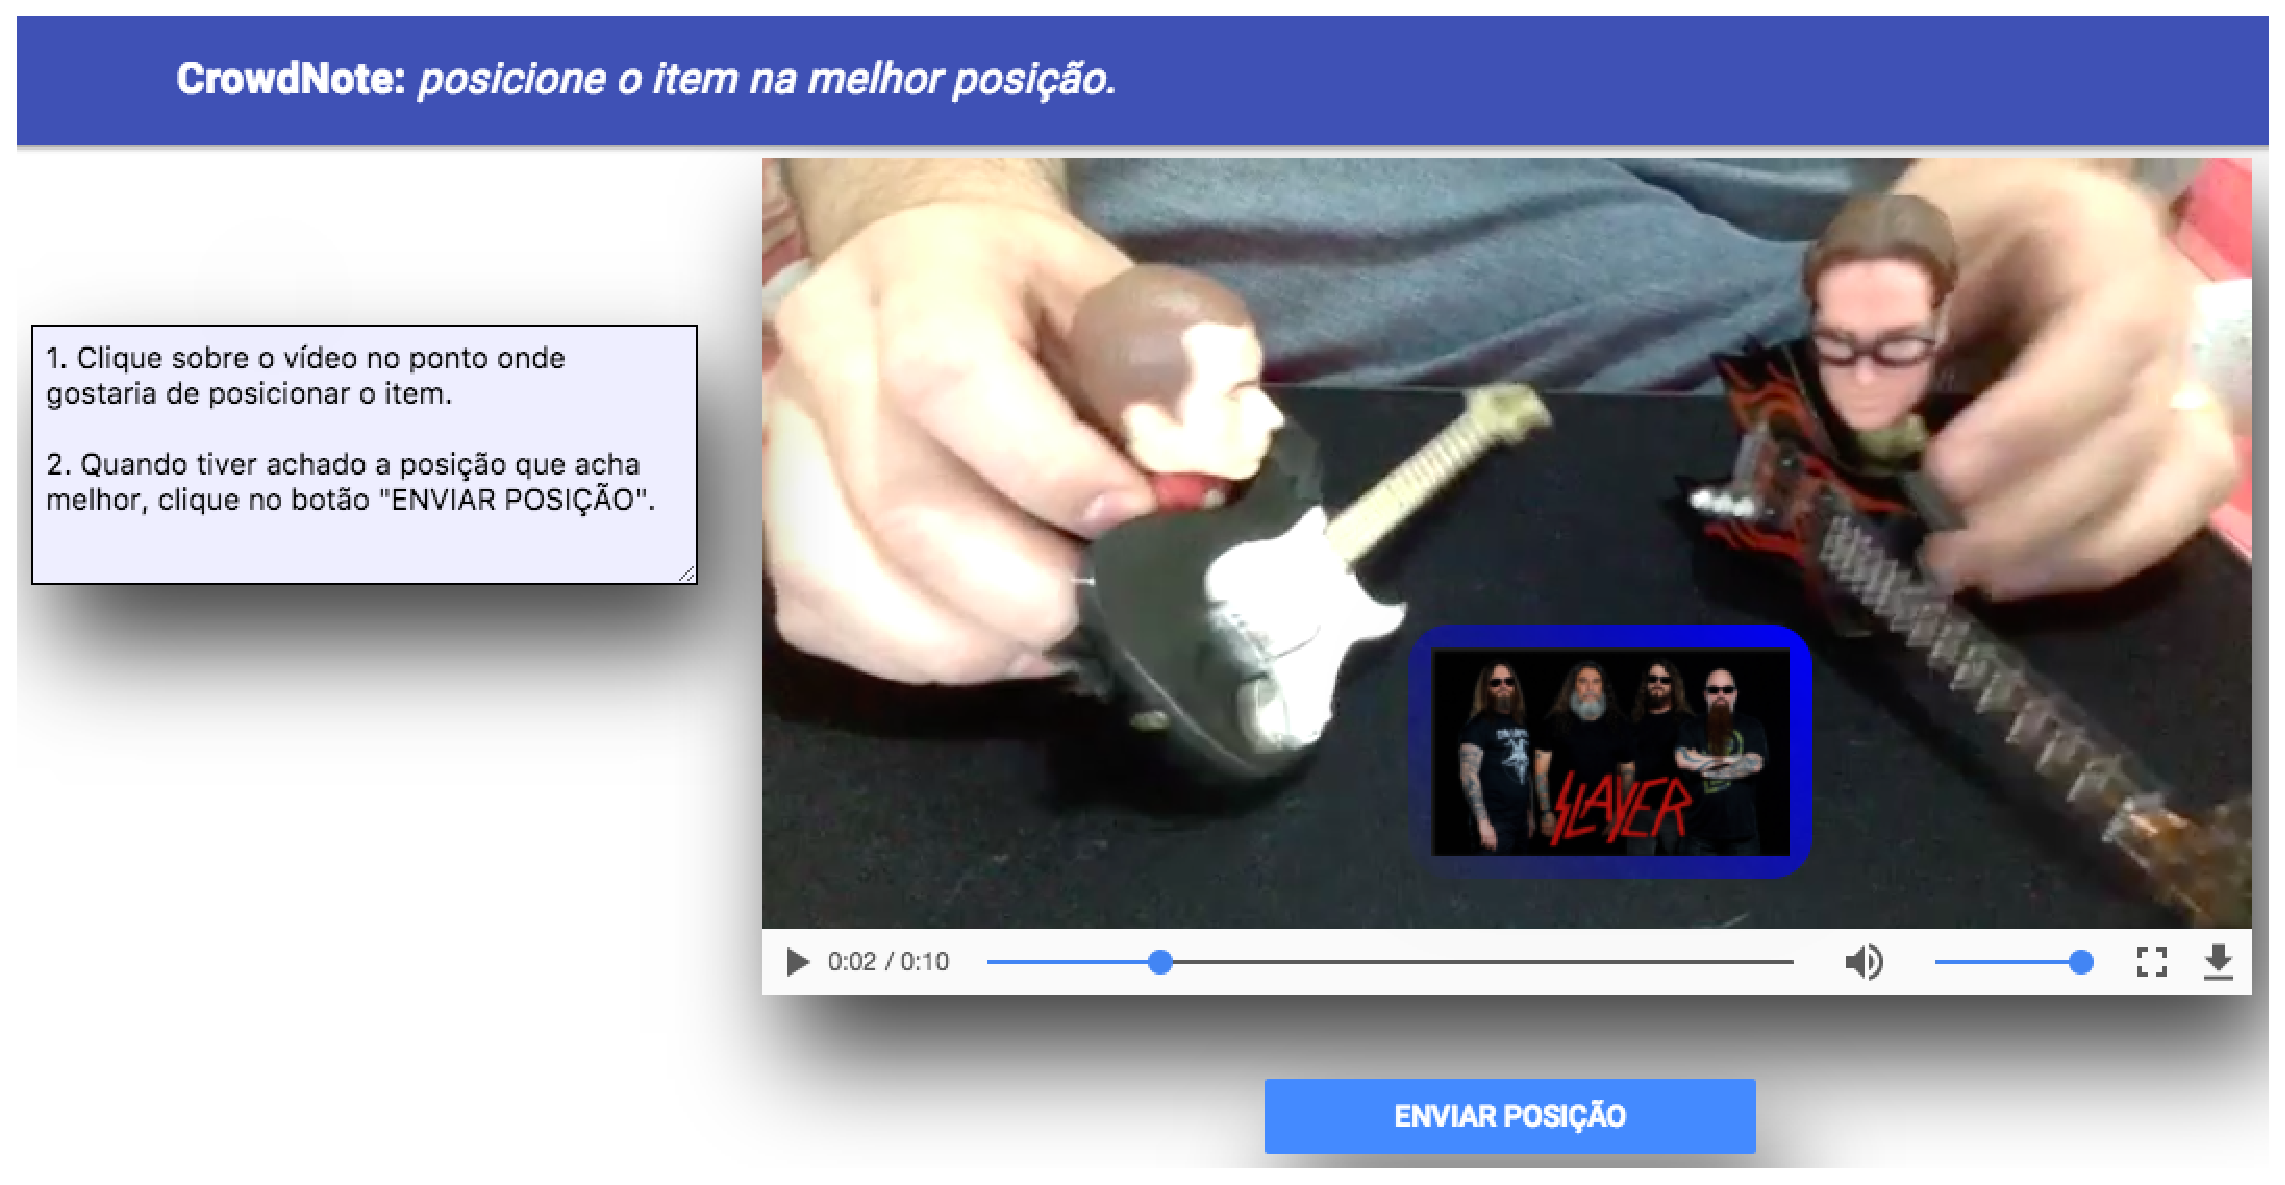
\includegraphics[scale=0.22] {figure/task_4}}
	\caption{Task 4}
	\label{task_4}
\end{figure}

\subsection{Player}

The presentation system, shown in Figure~\ref{player}, receives the video, extra content, and necessary meta-data from the Player Provider. This system is capable of reproducing the original video synchronized with the extra content, that is displayed every time a point of interest happen in the video. Actually, is important remind that all extra content displayed with the video was provided, selected and positioned by the crowd.

\begin{figure}[h!]
	\centerline{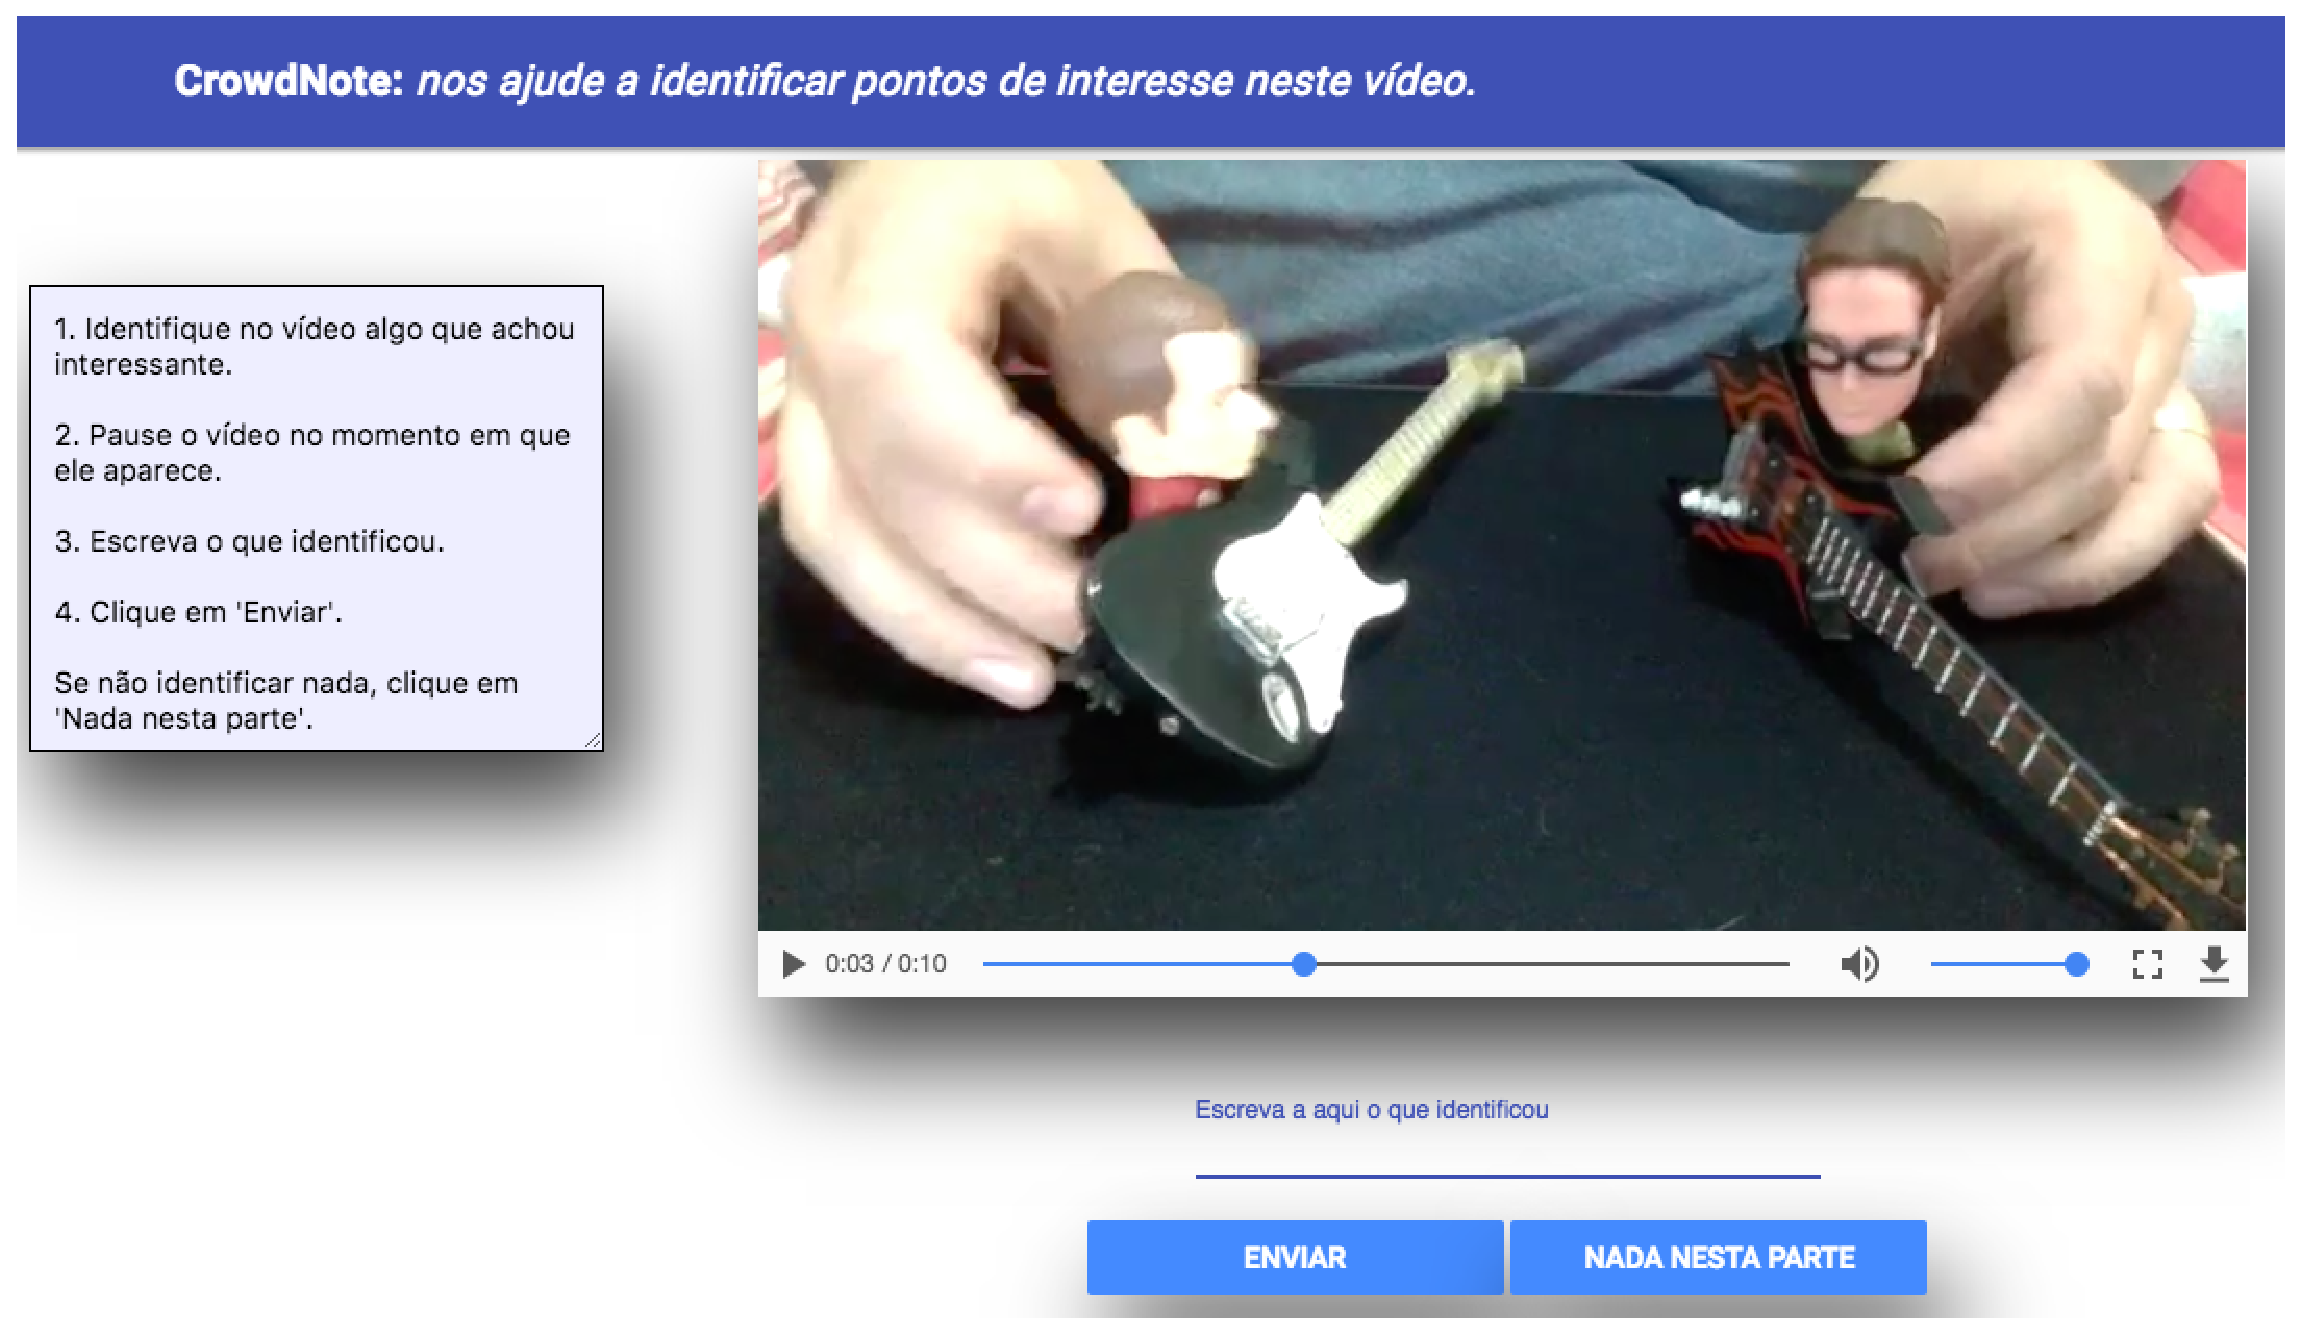
\includegraphics[scale=0.22] {figure/task_1}}
	\caption{Player}
	\label{player}
\end{figure}

When the user clicks on some extra content displayed in the video, the presentation is paused and a larger preview for the selected content is displayed in the zoom box as shown in the Figure~\ref{zoom}. This systems features navigation by extra-content instead the traditional timeline navigation, making available a button-bar with buttons to navigate among the extra contents.
 
\begin{figure}[h!]
	\centerline{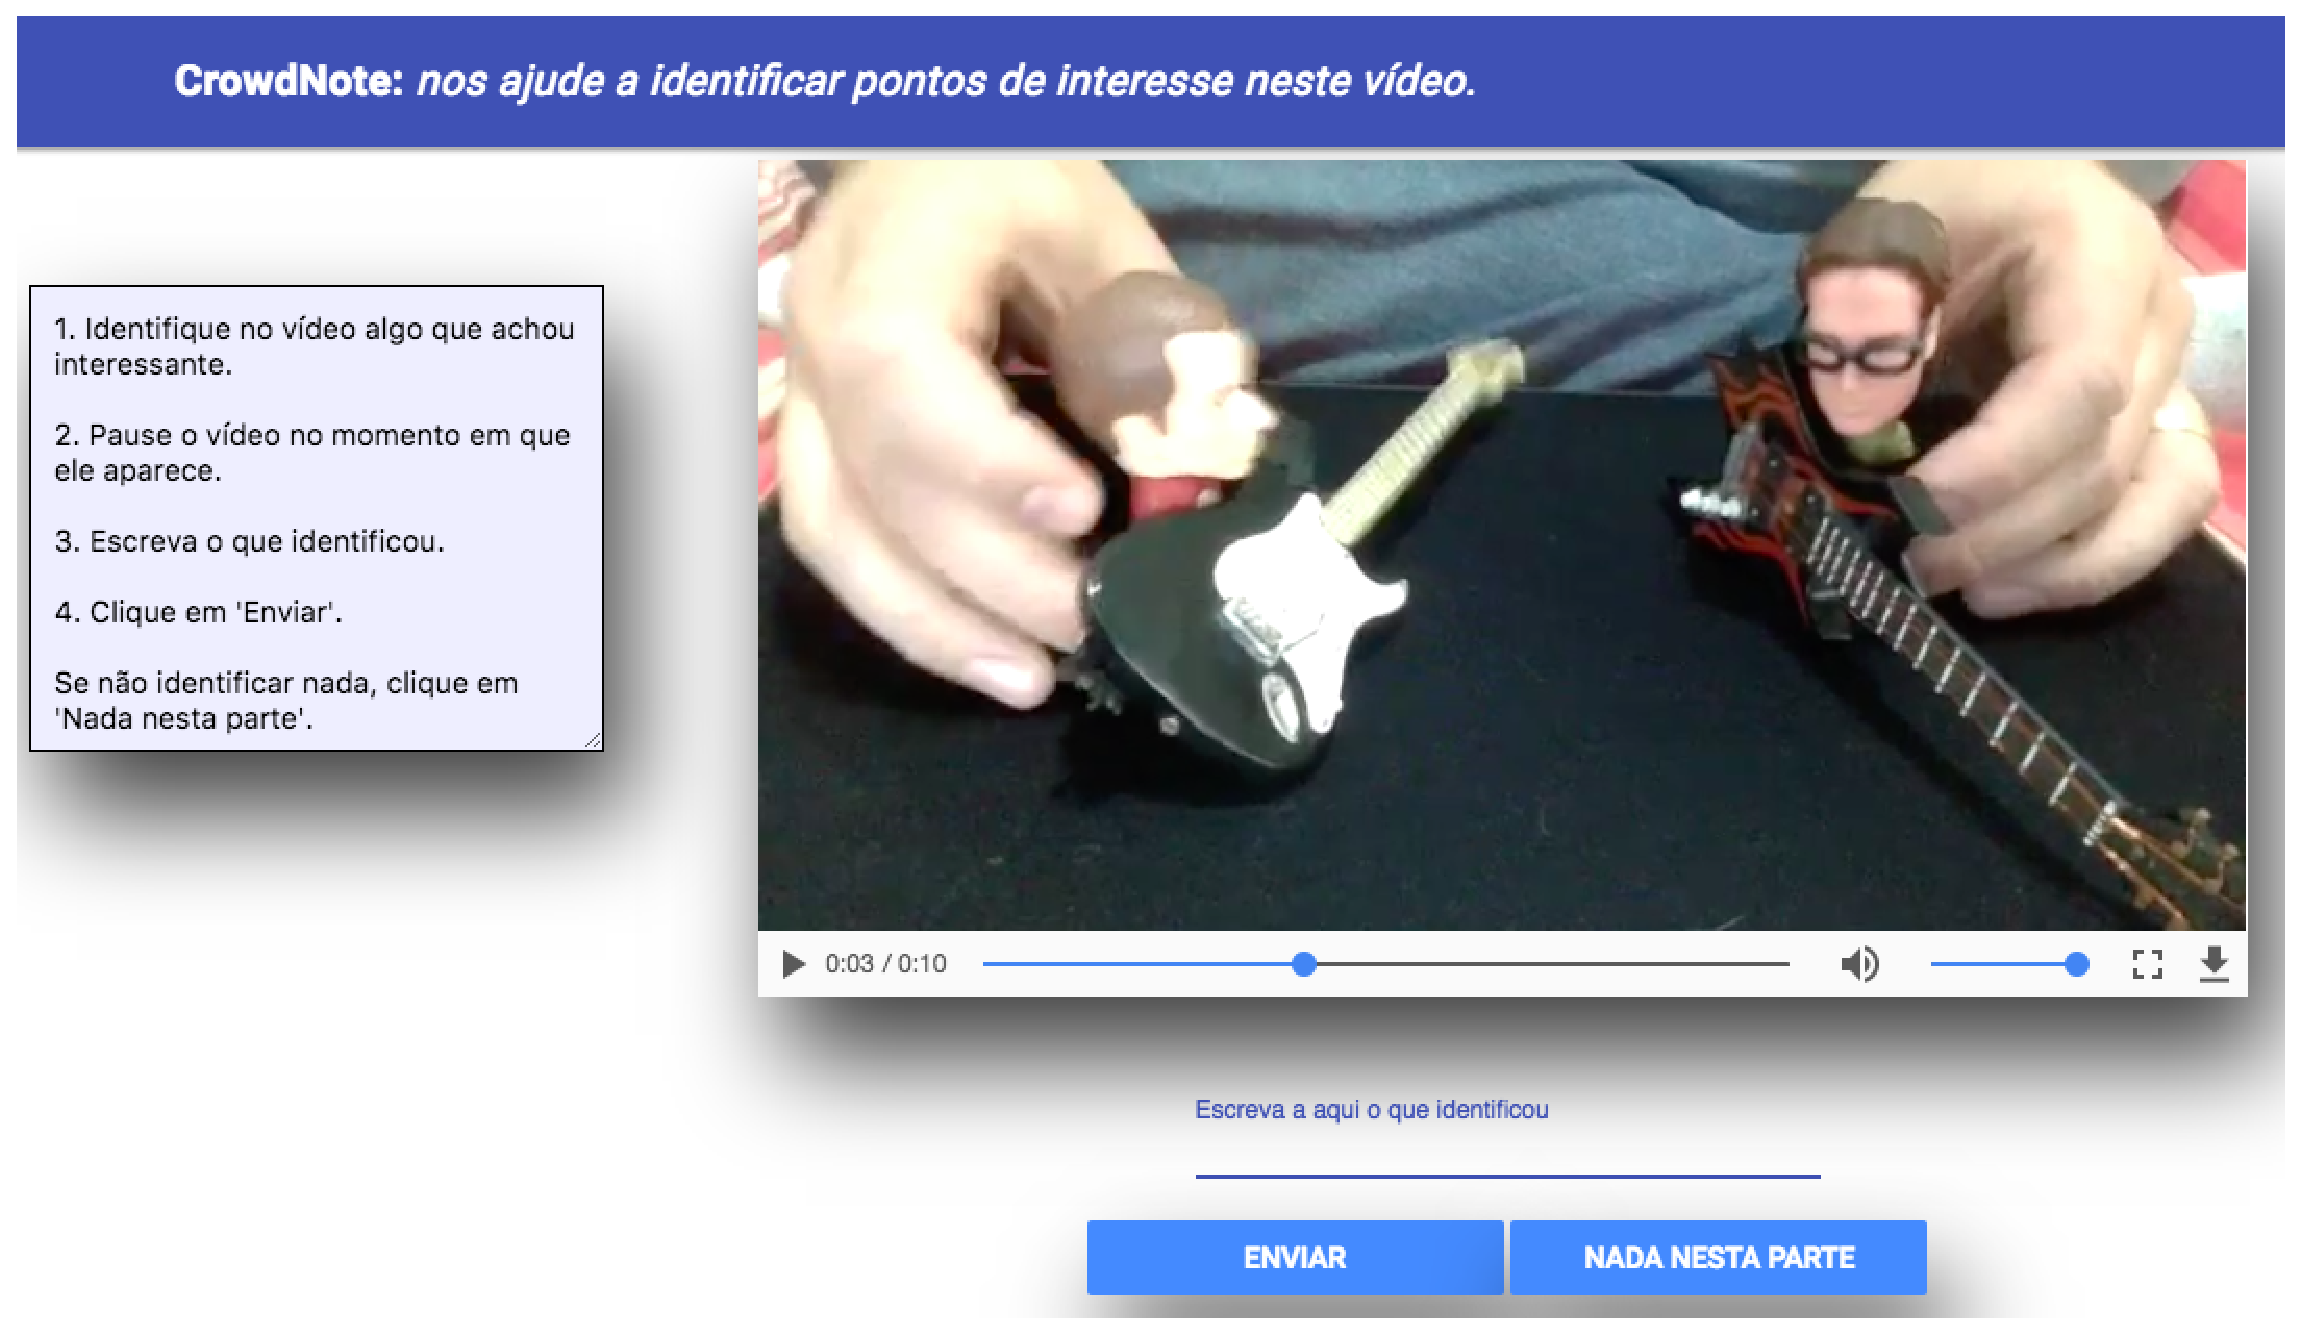
\includegraphics[scale=0.22] {figure/task_1}}
	\caption{Player}
	\label{zoom}
\end{figure}

	
\section{Job Router}
	The method used for the distribution of jobs among workers was defined according to two main criteria: 1. In each task, a worker can not contribute more than once to the same item; 2. It is desirable to obtain homogeneous coverage for items with similar amounts of contributions.

To meet the first requirement, the fingerprint of each worker is captured. This fingerprint is generated from the IP address and the signature of the Web browser. In this way, the system does not send the worker a job with an item he has already contributed.

The solution found to achieve a relatively homogeneous coverage of the items to be annotated, was adopted a routing strategy based on FIFO (first in first out) and LIFO (last in first out) structures, in accordance with the following rules:


\begin{itemize}

\item For each task, initially the items to be annotated are inserted into the entry LIFO.

\item For each job request, items are removed from the entry LIFO until an item that has not yet been annotated by the worker is found.

\item Items that have already been annotated by the worker are inserted into a temporary FIFO, which are re-entered into the entry LIFO when is found an item that still was not annotated by the worker.

\item When a worker has already annotated all the items, he is directed to a thank you page and receives no more items for that task.

\item Items taken from the entry LIFO and separated to be annotated, are inserted into the exit LIFO.

\item When the entry LIFO is empty, it is replenished by the exit LIFO, preserving an original order as far as possible.

\end{itemize}

This strategy aims to avoid that an item already annotated by a worker needs to wait until the next round is marked by another contributor. Initially, the use of a circular FIFO was considered. However, in a crowdsourcing environment, it would be very expensive to create mechanisms so that the elements already annotated by one worker would not sink until the end of the FIFO, losing the chance of being annotated by another worker in that round.

	
\section{Final Remarks}
	This paper presented CrowdNote, a crowdsourcing environment that can achieve complex video annotation from a crowd of untrained and nonspecializing contributors. CrowdNote can be used as template for different kinds of crowdsourcing applications based on video annotation.

To demonstrate how CrowdNote works, was created an instance of it that consists of a video enrichment application. This application used the crowd to annotate the points of interest present in the video, collect extra content to associate with them, select the collected content, and positionate the extra content in the video when each point of interest happens.

However, various types of applications can be generated as instances of CrowdNote. It is possible to create applications to annotate multiple aspects of scenes, generate transcriptions, human translations, among others.

The most interesting aspect of CrowdNote is that it offers a way to make complex video annotations without the work of experts, without the need to create expensive and sophisticated annotation systems, or ask employees to perform difficult and laborious tasks.

Traditional crowdsourcing approaches are struggling to achieve these complex annotations, but the strategy of dividing the problem into microtasks that collect simple annotations and cascades them to generate complex annotations proved to be functional.

Future versions of CrowdNote will incorporate features to assist the owner in generating bootstrap input, as well as selecting aggregation methods and annotation tools from a sample library.

The CrowdNote instance built for this work can be freely download, used and modified from GitHub [Removed for double-blind review] . 



\begin{acks}
Removed for double-blind review.
\end{acks}

\bibliographystyle{ACM-Reference-Format}
\bibliography{refs} 

\end{document}
